\section{kinematics tests}
Both forward and inverse kinematics are tested against Peter Corke's Robotics Toolbox MATLAB, use script $test\_kinematics$. \\
\textbf{\textcolor{red}{IMPORTANT:}} for the test it is required that \href[]{https://petercorke.com/toolboxes/robotics-toolbox/}{\textcolor{blue}{Peter Corke's Robotics Toolbox}} is installed. 
This is because we used the result from this toolbox as the ground truth.\\ 

Usage:\\
\texttt{>> test\_kinematics}\\
\subsection{Direct kinematics test}
Ten randomly generated joint angles are used to test the direct kinematics. We have used tolerance of $1e_-6$, 
and for this tolerance all the tests are passed. The test result is shown in Figure \ref{fig:direct_kinematics_test}.
\begin{figure}[H]
    \centering
    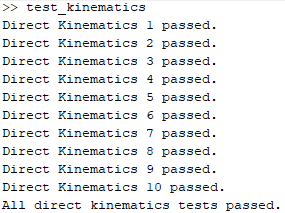
\includegraphics[width=0.4\textwidth]{images/direct_kinematics_test.png}
    \caption{Direct kinematics test}
    \label{fig:direct_kinematics_test}
\end{figure}

\subsection{Inverse kinematics test}
Similarly, ten homogeneous transformation matrices generated from 10 randomly generated joint angles 
are used to test the inverse kinematics. 
After calculating the inverse kinematics we recalculate the homogeneous transformation matrix and compare it with 
the original homogeneous transformation matrix. The same tolerance of $1e_-6$ is used and all the tests are passed.
The test result is shown in Figure \ref{fig:inverse_kinematics_test}.
\begin{figure}[H]
    \centering
    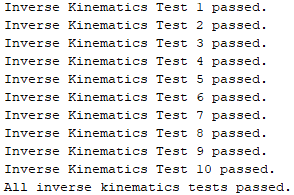
\includegraphics[width=0.4\textwidth]{images/inverse_kinematics_test.png}
    \caption{Inverse kinematics test}
    \label{fig:inverse_kinematics_test}
\end{figure}